% main.tex — Journal of Neural Engineering (IOP iopjournal sınıfı). Taslak iskelet v1 (2026-10-02).
% Bölümler sections/ altında; tablolar PyCharm'ın ürettiği tables/*.tex dosyaları; şekiller figures/ altında.
\documentclass{iopjournal}

\usepackage{amsmath}
\usepackage{booktabs}

\begin{document}

\articletype{Paper}

\title{High accuracy without demonstrated generalization: data leakage and recording confounds in resting-state EEG classification of juvenile offenders}

\author{Mesut Melek$^{1}$\orcid{0000-0002-7152-7788} and Negin Melek$^{2,*}$\orcid{0000-0001-5297-5545}}

\affil{$^1$Department of Software Engineering, Faculty of Engineering, G\"um\"u\c{s}hane University, G\"um\"u\c{s}hane, T\"urkiye}

\affil{$^2$Department of Electrical and Electronics Engineering, Faculty of Engineering, G\"um\"u\c{s}hane University, G\"um\"u\c{s}hane, T\"urkiye}

\affil{$^*$Author to whom any correspondence should be addressed.}

\email{negin.melek@gumushane.edu.tr}

\keywords{EEG, data leakage, cross-validation, juvenile offenders, confounds, resting state, generalization}

\begin{abstract}
[ABSTRACT: Objective, Approach, Main results, Significance; at most 300 words. Written last.]
\end{abstract}

\section{Introduction}
\label{sec:intro}
[INTRODUCTION: written after the Methods, Results and Discussion.]

% sections/methods.tex — Yöntem bölümü, taslak v1 (2026-10-02)
% Kaynaklar: CLAUDE.md (2026-10-02), 02 v2 raporu, 03 planı v2, 04_05 planı v2, 04-B planı v1,
% Tablo S-n v2, iskelet v6. Köşeli parantezli büyük harfli yerler henüz doldurulmadı.

\section{Methods}
\label{sec:methods}

Analysis identifiers in parentheses (03--07g) refer to the analysis log (table~S2) and to the code repository.

\subsection{Dataset and participants}
\label{sec:data}

We analysed the openly available dataset ``Dataset of Electroencephalograms of Juvenile Offenders'' (OpenNeuro ds006923, version 1.0.0, CC0 licence) \cite{Polo2025ds006923}. It contains resting-state EEG recordings of 140 male adolescents: 74 juvenile offenders, labelled as two subgroups (sg, $n = 49$; sg2, $n = 25$), and 66 controls without a criminal record (cg). Demographic, educational, substance-use and offence variables were taken from the dataset's participants file (table~\ref{tab:Table1}).

The dataset documentation does not define the two offender labels. A conference report from the same data-collection project describes the 74 offenders as 50 young people confined in a rehabilitation centre and 24 under non-custodial pedagogical measures \cite{RodriguezAlvarez2023}. Whether these two groups correspond to sg and sg2 cannot be verified from the published metadata. We therefore kept the dataset labels throughout.

Data collection was approved by the Ethics Committee of Universidad del Magdalena \cite{Polo2025ds006923}; for the same project, the approval date is reported as 23 May 2019, and informed consent was obtained from all participants, with the consent of parents or legal guardians for those under 18 \cite{SanchezTorres2024}. The present study is a secondary analysis of de-identified open data and required no further ethical approval.

\subsection{Recording and preprocessing by the data providers}
\label{sec:recording}

EEG was recorded with a BioSemi ActiveTwo system (128 scalp channels, 2048~Hz) \cite{Polo2025ds006923,RodriguezAlvarez2023}. The resting protocol consisted of four 60-s blocks alternating eyes closed and eyes open (closed--open--closed--open), followed by an eyes-closed block of about 8~min. The providers preprocessed the data before publication: finite impulse response band-pass filtering (1--40~Hz), average reference, artifact subspace reconstruction \cite{Mullen2015}, independent component analysis with ICLabel classification \cite{PionTonachini2019}, and downsampling to 128~Hz. Electro-oculographic and electrocardiographic channels were recorded \cite{RodriguezAlvarez2023} but are not included in the published files.

For each participant, the dataset provides the full preprocessed recording and an epochs file with four 50-s segments (two eyes closed, two eyes open). We verified that each segment is an exact excerpt of the preprocessed recording that starts 5~s after its block marker (difference 0~$\mu$V). Analyses of the four segments therefore used the epochs files, and analyses of the long eyes-closed block used the preprocessed recordings.

\subsection{Data audit and analysis samples}
\label{sec:audit}

All 140 recordings were audited before any group comparison: file integrity, duration, block markers and channel count. Five participants lacked the long eyes-closed block. Four sg participants had only about 157~s of data (one eyes-closed and one eyes-open block), and the preprocessed recording of sub-1084sg2 could not be read because its data file is not part of the published dataset. The long-block sample therefore comprised 135 participants (cg 66, sg 45, sg2 24). The alpha-reactivity analysis needs only the four 50-s segments and comprised 136 participants (cg 66, sg 45, sg2 25); the four short sg recordings entered a sensitivity analysis ($n = 140$). The sample of every analysis is given in table~\ref{tab:TableSn} and figure~\ref{fig:cohort}.

The audit also extracted the recording date and clock time of each session from the acquisition time stamps (table~\ref{tab:Table1}). The site field of the published sidecar files lists the same institution for all 140 participants, controls included; we therefore treated it as uninformative.

\subsection{Analysis log, preregistration status and use of AI tools}
\label{sec:log}

The analyses were not preregistered. Every analysis plan, decision rule and change was recorded in a time-stamped analysis log (a project file, written analysis plans and the git history). Table~S2 lists all decisions and states for each whether it was made before the relevant result was seen.

The single primary test (alpha reactivity; section~\ref{sec:primary}) was designated after the batch negative control (section~\ref{sec:negcontrol}) had been run. Before this designation, 42 unadjusted univariate comparisons of the 14 region-of-interest (ROI) features had been inspected; alpha reactivity was not among them, and these comparisons informed no feature selection (table~S2). The definitions of the last two exploratory analyses (07f, 07g) were committed to the repository in separate commits before they were run; the commit contents are provided as supplementary files. For earlier steps, the order of definition and result rests on the analysis log; for 07d and 07e, definition and results share one commit.

The analysis code was written and executed by an AI coding agent (Claude Code, Anthropic; model Claude Opus 5.5) under the authors' direction. The authors approved every analysis plan, decision rule and interpretation. Four audits of code, numbers and text were carried out in separate sessions of the same model (Claude Opus 5.5); these audits are therefore not independent. Their findings and the resulting corrections are listed in table~S2. The authors take full responsibility for the analyses and the text.

\subsection{Spectral features}
\label{sec:features}

Feature parameters were fixed before any group comparison (table~\ref{tab:TableS3}). From the long eyes-closed block, we analysed a fixed 465-s segment starting 5~s after the third eyes-closed marker, and its two halves (H1 and H2, 232.5~s each). Power spectral density was estimated with Welch's method (4-s Hann windows, 50\% overlap, 0.25-Hz resolution). Relative band power was computed for delta (1--4~Hz), theta (4--8~Hz), alpha (8--13~Hz) and beta (13--30~Hz) as a fraction of total 1--30~Hz power. The aperiodic exponent and offset were estimated with FOOOF version~1.1 \cite{Donoghue2020} in the `fixed' aperiodic mode over 3--30~Hz; a `knee' fit over 2--30~Hz was used only as a sensitivity analysis. The individual alpha frequency (IAF) was defined as the strongest FOOOF peak between 7 and 13~Hz (primary) and as the centre of gravity of the aperiodic-removed spectrum between 7 and 13~Hz (secondary).

Channels were excluded within each participant if the FOOOF fit had $R^2 < 0.9$ or if an electromyographic (EMG) index exceeded a robust $z$ score of 3 (one-sided; median $+\,3 \times 1.4826 \times$ median absolute deviation). The EMG index was the slope of log power against log frequency over 30--40~Hz; flatter slopes indicate more muscle activity. Because the providers' low-pass filter also shapes this slope, the index was used only as a relative measure. ROI features were computed from the mean spectrum of the retained channels in a posterior ROI (nine channels: [ROI CHANNEL LIST]) and in a global ROI (all retained channels).

One rule was added after inspection of quality-control data but before any group comparison: participants with more than 25\% of channels excluded were flagged as having an atypical spectrum, and only the EMG rule was applied to them. Two sg2 participants were flagged (88 and 57 channels excluded by the $R^2$ rule). They were kept in the primary analyses and excluded in sensitivity analyses. When the rule was adopted, it was known that both belonged to sg2 and used cannabis and cocaine (table~S2).

Vigilance was indexed by the slope of the log$_{10}$ theta/alpha ratio across consecutive 30-s windows of the long block; a positive slope indicates increasing drowsiness \cite{Strijkstra2003}. The 14 ROI features used in the ROI-level analyses were relative delta, theta, alpha and beta power, the aperiodic exponent and offset, and the primary IAF, each in the posterior and global ROIs.

\subsection{Batch negative control (03)}
\label{sec:negcontrol}

Before any offender--control comparison, we asked (a) whether the 14 ROI features separate the two offender subgroups (sg vs sg2) and (b) whether a model trained on sg vs cg also separates sg2 from cg. A preliminary comparison showed that sg and sg2 differ not only in recording period but also in offence profile, alcohol use and age (table~\ref{tab:Table1}). A positive result in (a) could therefore not be read as a pure batch effect.

The pipeline was median imputation, standardisation and L2-regularised logistic regression with balanced class weights, all fitted within training folds. Each participant contributed one row. The outer loop was stratified 5-fold cross-validation repeated 20 times; an inner stratified 5-fold loop selected the regularisation strength (13 values from $10^{-3}$ to $10^{3}$) by area under the ROC curve (AUC). In (b), the model of each outer fold scored that fold's held-out controls and all 24 sg2 participants, and the AUC of sg2 versus the held-out controls was computed within the fold and averaged over the 100 folds. For both tests, labels were permuted 1000 times and the full nested procedure was rerun with 5 repeats per permutation; $p = (k+1)/(N+1)$ and $\alpha = 0.025$ per test (Bonferroni). Six prespecified sensitivity analyses repeated the pipeline without permutation: excluding the two atypical participants; regressing the EMG index and the vigilance slope, or age, out of each feature within training folds; using H1 instead of the full segment; omitting the aperiodic offset; and using the knee-model features.

\subsection{Leakage demonstration on the published features (04-A, 04-B)}
\label{sec:leakage}

The dataset also contains precomputed features: 2048 spreadsheet files (four bands $\times$ four segments [C1, O1, C2, O2] $\times$ 128 channels), each with seven statistics per participant, and an equivalent MATLAB file. We first audited these files (04-A): consistency across files, column quality, internal consistency of the statistics, and the identity of the 112 participants they contain (cg 66, sg 46; no sg2). Identity was checked by correlating each participant's standardised log-power profile in the spreadsheets with the same profile recomputed from the published epochs files (table~\ref{tab:TableS5}).

We then quantified leakage with these features as published (04-B): 448 rows (112 participants $\times$ 4 segments) with 3584 features each. A $2 \times 2$ design crossed the cross-validation unit (row-wise stratified 10-fold vs subject-wise 5-fold) with the place of feature selection (ANOVA $F$ test, top 100 features, on all data vs within training folds). This gives four non-nested pipelines, N1--N4, each repeated with 10 random seeds; N1, with row-wise splits and selection on all data, represents a common naive approach. We built these naive pipelines to illustrate the error; they do not reproduce any published analysis of these data. The correct pipeline (P) was nested and subject-wise: an outer stratified group 5-fold loop repeated 20 times and an inner stratified group 5-fold loop that selected the number of features ($k \in \{10, 50, 100, 500\}$) and, for the support vector machine, $C \in \{0.1, 1, 10\}$. Classifiers were a support vector machine with a radial basis function kernel and a random forest with 500 trees; standardisation was always fitted within training folds. A participant's score was the mean of its row scores. Subject-level AUC was the primary metric; row-level AUC, balanced accuracy and Golden Distance were secondary.

To show how much performance arises without signal, labels were permuted at the subject level 200 times for N1 (both classifiers) and for P (support vector machine, 5 repeats per permutation). Sensitivity analyses used only the 100 identity-verified participants, removed the kurtosis features, or used only the eyes-closed segments.

\subsection{Primary hypothesis test: alpha reactivity (05)}
\label{sec:primary}

The single primary test compared the posterior alpha reactivity index (ARI) between offenders (sg and sg2 combined) and controls. Absolute alpha power (8--13~Hz; Welch's method as above) was computed in each of the four 50-s segments of the first 4~min and averaged over the nine posterior channels, omitting each participant's excluded channels (section~\ref{sec:features}; all nine channels for sub-1084sg2). With $C$ and $O$ the mean alpha power of the two eyes-closed and the two eyes-open segments, $\mathrm{ARI} = (C - O)/(C + O)$. Because the index is a ratio, multiplicative gain differences cancel.

The test was a two-sided Mann--Whitney $U$ test ($\alpha = 0.05$; 70 offenders, 66 controls). Effect sizes were the rank-biserial correlation and the Hodges--Lehmann shift \cite{HodgesLehmann1963}, each with a bootstrap 95\% confidence interval (CI; 2000 resamples). In a covariate sensitivity analysis, ordinary least-squares models regressed the ARI, and separately its ranks, on group, age and the posterior EMG index from the same segments, with HC3 standard errors \cite{MacKinnonWhite1985}. A second sensitivity analysis added the four short sg recordings, using their single eyes-closed and eyes-open segments ($n = 140$). The interpretation was fixed in advance: a positive result would be reported as a group difference not explained by gain but not separable from substance use, recording period or site; a negative result would be quantified by its CIs.

\subsection{Quantifying the ROI-level null result (06)}
\label{sec:null}

Offenders (sg and sg2 combined, $n = 69$) and controls ($n = 66$) were classified with the 14 ROI features and the pipeline of section~\ref{sec:negcontrol}. Each participant's out-of-fold probability was averaged over the 20 repeats. The AUC of these averaged scores received a 95\% CI from a class-stratified participant bootstrap (2000 resamples, percentile) and, as a cross-check, from DeLong's method \cite{DeLong1988}. This CI does not include variability from model training; the 2.5th--97.5th percentile range of the per-repeat AUCs is reported separately. The upper CI limit was taken as the smallest effect that is approximately excluded and was converted to Cohen's $d = \sqrt{2}\,\Phi^{-1}(\mathrm{AUC})$.

\subsection{Exploratory channel-level analyses (07--07g)}
\label{sec:exploratory}

After the ROI-level analyses, a series of exploratory analyses asked whether channel-level spectral features separate sg from controls and whether such a separation transfers to sg2. For comparability with the leakage analysis, these analyses used the 100 identity-verified participants of the spreadsheet cohort (sg 45, cg 55), with features computed from the published recordings. Two feature sets were computed per segment and channel (Welch's method as above; 128 channels $\times$ 4 bands = 512 features): (A) log$_{10}$ absolute band power and (B) relative band power. All analyses used pipeline P with the support vector machine (section~\ref{sec:leakage}) and 200 subject-level label permutations with 5 repeats each. Their $p$ values are not adjusted for multiple comparisons.

\begin{itemize}
  \item 07: sets A and B on all four segments. Separation in A but not in B was to be attributed to absolute amplitude.
  \item 07a: set B on the eyes-closed and the eyes-open segments separately. 07b: set B on the eyes-closed segments without the 32 channels of the BioSemi C block, which covers frontopolar, anterior frontal and right frontal sites (equivalents include Fp1, Fpz, Fp2, AF7, AF3, AFz, AF4, AF8, F1, Fz, F2, F4, F6, F8, FC1, FCz and FC2).
  \item 07c and 07d: transfer to sg2 ($n = 24$) of the eyes-closed model (07c) and of the three strongest segment models (set A on all segments, set B on all segments and set B on the eyes-open segments; 07d). Transfer was measured with the within-fold AUC of section~\ref{sec:negcontrol}; the permutation null shuffled the training labels.
  \item 07e: the long eyes-closed block (the 465-s segment of section~\ref{sec:features}) divided into four consecutive, non-overlapping 116.25-s parts, set B, without channel exclusion. 07f: transfer of the 07e model to the long blocks of sg2 ($n = 24$).
\end{itemize}

The decision rule of 07a--07c combined an AUC threshold with $p < 0.05$ and left the interval 0.60--0.65 undefined; 07d--07f used a single criterion, permutation $p < 0.05$. For the transfer tests, $p < 0.05$ in any model would have narrowed the claim of this paper; without multiplicity correction, this rule is conservative for the claim that there is no evidence of transfer.

Analysis 07g quantified uncertainty without a decision rule. For the six source models (07 A, 07 B, 07a eyes closed, 07a eyes open, 07b and 07e), each participant's decision value was averaged over the 20 repeats, and the AUC of these averaged scores received a 95\% CI from a class-stratified participant bootstrap (2000 resamples). For the five transfer models (07c, three 07d models and 07f), a weighted participant bootstrap drew multinomial weights for the controls and for sg2, shared them across all folds of a resample, recomputed each fold's AUC as a weighted Mann--Whitney statistic and averaged over the 100 folds (2000 resamples, percentile). Before the CIs were computed, all 1120 reproduced AUCs were checked against the saved values (maximum difference $6 \times 10^{-17}$). These CIs reflect participant sampling only. A descriptive map of the 07e contrast (Hedges' $g$ for each channel and band; no test) is shown in figure~\ref{fig:S07e}.

\subsection{Statistics, metrics and software}
\label{sec:stats}

The AUC was the primary classification metric; balanced accuracy and the Golden Distance (GD) were secondary. GD summarises three or more performance metrics in a single score \cite{Melek2025GD}. We used accuracy, sensitivity, specificity and F1 with the offender class as positive, for which the GD polygon is a square; lower values indicate performance closer to the ideal. Permutation $p$ values were computed as $(k+1)/(N+1)$ \cite{Ojala2010}; with 200 permutations the smallest attainable value is $1/201$, reported as $p \le 0.005$. Ranges across cross-validation repeats (2.5th--97.5th percentile) describe training variability and are not confidence intervals. Exploratory $p$ values are not adjusted for multiple comparisons. AUCs and CIs are given with two decimals in the text, because the bootstrap limits vary by about $\pm 0.01$ with the random seed, and $p$ values with three decimals. Random seeds were fixed (20261001).

Analyses were run in Python with scikit-learn \cite{Pedregosa2011}, FOOOF \cite{Donoghue2020} and [OTHER PACKAGES AND VERSIONS]. The code, the analysis log and all result files are available at [REPOSITORY / ZENODO DOI].


% sections/results.tex — Bulgular bölümü, taslak v1 (2026-10-02)
% Sayıların kaynakları: Tablo 1, 2, 3, 4, S4, S5, S_leak (09 v3/v4, kayıtlı CSV'lerden), CLAUDE.md, DENETIM_RAPORU 1–4.
% Kural: AUC ve güven aralıkları iki ondalık, p değerleri üç ondalık.

\section{Results}
\label{sec:results}

\subsection{Cohort, confounds and data integrity}
\label{sec:res-cohort}

Offenders and controls differed in most recorded characteristics (table~\ref{tab:Table1}). Cannabis and cocaine use were reported by 74\% and 66\% of offenders and by no control, and 81\% of offenders but no control had left school. Offenders were older ($17.0 \pm 1.1$ vs $16.3 \pm 1.1$ years) and of lower socioeconomic stratum (both $p < 0.001$).

Group was also confounded with recording period (figure~\ref{fig:cohort}; table~\ref{tab:Table1}). sg was recorded in July--September 2021, sg2 between December 2021 and June 2022, and the controls between February and September 2022. sg and the controls shared no recording month, and sg2 and the controls overlapped only in May--June 2022 (11 sg2 and 9 control recordings). Mean recording clock time was similar across groups (11.5--11.9~h), but recordings after 14:00 were more frequent in sg (29\%) and sg2 (28\%) than in the controls (9\%; offenders vs controls $p = 0.005$). The two offender subgroups also differed in offence profile (violent primary offence: sg 86\%, sg2 24\%; $p < 0.001$), in alcohol use (51\% vs 80\%; $p = 0.023$) and in age ($p = 0.031$).

The precomputed spreadsheet features did not correspond to the published recordings (table~\ref{tab:TableS5}). All 2048 files describe the same 112 participants (66 cg and 46 sg, no sg2). Twelve spreadsheet identifiers have no published recording, and 40 published participants are absent from the spreadsheets (all 25 sg2, 4 sg and 11 cg). Every statistic in the files except power was computed from exactly three values: kurtosis equals 1.5 in every cell, which is the kurtosis of any three distinct values, and the largest absolute skewness equals the three-value bound of $1/\sqrt{2}$ (supplementary note S1). For the 100 participants present in both sources, each spreadsheet profile correlated best with the participant's own recording (median $r = 0.92$, range 0.72--0.98). None of the 12 unmatched identifiers matched a published recording (best $r$ 0.25--0.66).

\subsection{Data leakage inflates classification performance}
\label{sec:res-leakage}

With the naive pipeline (N1), the published features separated offenders from controls with a subject-level AUC of 0.91 (random forest) and 0.89 (support vector machine), and a subject-level balanced accuracy of 0.80 and 0.76 (table~\ref{tab:Table2}; figure~\ref{fig:leakage}). Most of this performance did not depend on the labels. After subject-level label shuffling, N1 still reached a subject-level AUC of 0.85 and 0.79 (row-level 0.78 and 0.73; $p \le 0.005$ for the real labels). The correct nested pipeline (P) reached 0.73 with the random forest (repeat range 0.67--0.79) and 0.66 with the support vector machine (repeat range 0.59--0.75; shuffled-label null 0.48, $p = 0.010$).

In the $2 \times 2$ decomposition (row-level AUC; differences computed from unrounded values), splitting by row rather than by participant added 0.21--0.22 (N2 vs N4; row-wise splits used 10 folds and subject-wise splits 5, so this difference also includes a small effect of training-set size). Selecting features on all data added 0.01--0.03 with row-wise splits (N1 vs N2) and 0.04--0.09 with subject-wise splits (N3 vs N4). The GD showed the same pattern: 0.38--0.44 for N1 and 0.64--0.68 for P (lower is better). The pattern held when only the 100 identity-verified participants were used (P: 0.69 and 0.62), without the kurtosis features, and with eyes-closed segments only (table~\ref{tab:TableS_leak}). Because the spreadsheet cohort differs from the published cohort and its features depend on absolute amplitude, we do not interpret the above-chance AUC of P as a group difference.

\subsection{Primary test: alpha reactivity did not differ}
\label{sec:res-primary}

Alpha reactivity did not differ between offenders and controls (table~\ref{tab:Table3}; figure~\ref{fig:primary}). The median ARI was 0.64 in offenders and 0.68 in controls ($U = 2114$, $p = 0.395$). The rank-biserial correlation was $-0.08$ (95\% CI $-0.28$ to 0.11) and the Hodges--Lehmann shift $-0.03$ ($-0.10$ to 0.04). Adjusting for age and the EMG index did not change the result (offender coefficient 0.01, 95\% CI $-0.07$ to 0.08, $p = 0.886$; rank model $p = 0.988$), nor did adding the four short recordings ($n = 140$, $p = 0.279$). Descriptively, the median ARI was 0.64 in sg, 0.62 in sg2 and 0.68 in the controls. Rank-biserial correlations below $-0.28$ or above 0.11 are therefore approximately excluded.

\subsection{Prespecified ROI features did not separate the groups}
\label{sec:res-roi}

With the 14 prespecified ROI features, offenders could not be distinguished from controls: AUC 0.54 (95\% CI 0.44--0.63; DeLong 0.44--0.64; repeat mean 0.51, range 0.46--0.57; table~\ref{tab:Table4}; figure~\ref{fig:roi}). For these features and this model, and considering participant sampling only, AUCs above 0.63 (Cohen's $d \approx 0.48$ under the equal-variance normal model) are approximately excluded; smaller effects are not.

The null result is not explained by the inclusion of sg2. The same features gave an AUC of 0.53 for sg versus controls (repeat range 0.43--0.63), and descriptively the out-of-fold scores of the offender model gave 0.55 for sg and 0.52 for sg2 against the controls. In the batch negative control, sg versus sg2 reached 0.63 (repeat range 0.54--0.71; $p = 0.053$, against $\alpha = 0.025$ and a significance threshold of 0.65), and a model trained on sg versus controls gave a within-fold AUC of 0.44 for sg2 versus held-out controls ($p = 0.771$). The prespecified sensitivity analyses gave similar values (sg vs controls 0.50--0.56; sg vs sg2 0.58--0.63; transfer 0.42--0.53).

\subsection{Exploratory: channel-level features separated sg from controls}
\label{sec:res-channel}

Channel-level spectral features separated sg from the controls in the 100 identity-verified participants (figure~\ref{fig:cascade}a; table~\ref{tab:TableS4}). On all four segments, log absolute power (set A) and relative power (set B) reached AUCs of 0.75 and 0.73 (both $p \le 0.005$; null mean 0.48), so the separation was not due to absolute amplitude alone. Relative power gave a higher AUC on the eyes-open segments (0.71, $p \le 0.005$) than on the eyes-closed segments (0.64, $p = 0.015$); the difference was not tested. Removing the 32 channels of the C block lowered the eyes-closed AUC to 0.58 ($p = 0.0498$). Because the eyes-closed AUC fell in the interval that the prespecified rule left undefined, the rule gave no verdict. In the long eyes-closed block, relative power separated sg from the controls with an AUC of 0.75 (repeat range 0.65--0.80; $p \le 0.005$). Across these analyses, the repeat-mean AUCs ranged from 0.64 to 0.75. AUCs computed from repeat-averaged scores are higher; for the long block, 0.78 (95\% CI 0.69--0.87; table~\ref{tab:TableS4}).

Single-feature differences in the long block were small to moderate ($|g| \le 0.58$; figure~\ref{fig:S07e}). All ten largest effects, and 18 of the 20 largest, were at C-block sites over frontopolar and anterior frontal cortex. sg showed higher relative delta power and lower theta and beta power; alpha power did not differ (median $g$ in the posterior A block 0.01).

The same groups in the same block thus gave an AUC of 0.53 with ROI features and logistic regression ($n = 111$) and 0.75 with channel features and the support vector machine ($n = 100$). These analyses differ in feature resolution, model, channel exclusion and sample, and the contributions of these choices were not separated.

\subsection{Exploratory: no evidence of transfer to sg2}
\label{sec:res-transfer}

None of the five models trained on sg versus controls showed significant transfer to sg2 (figure~\ref{fig:cascade}b; table~\ref{tab:TableS4}). The within-fold transfer AUCs (sg2 vs held-out controls) were 0.57 for the eyes-closed model (95\% CI 0.44--0.69; $p = 0.264$); 0.55 (0.44--0.66; $p = 0.224$), 0.59 (0.48--0.70; $p = 0.194$) and 0.55 (0.45--0.66; $p = 0.289$) for the three strongest segment models; and 0.58 (0.46--0.70; $p = 0.104$) for the long-block model. Under the prespecified rule, the claim of no evidence of transfer therefore holds for all five models.

To be significant, a transfer AUC would have had to exceed 0.59--0.64 (the one-sided 95th percentile of the null). Considering participant sampling only, the upper CI limits of 0.66--0.70 approximately exclude transfer AUCs above about 0.70 for these models, but moderate transfer cannot be excluded: the data are compatible with anything from no transfer to moderate transfer. Without the two atypical sg2 participants (descriptive; no CI), the transfer AUCs were 0.53--0.57; they rose only for the set-A model (from 0.55 to 0.57) and fell by 0.02--0.03 for the other four. The difference between source and transfer AUCs was not tested.


% sections/discussion.tex — Tartışma ve Sonuç bölümleri, taslak v1 (2026-10-02)
% Kaynaklar: iskelet v6 (Tartışma, Sınırlılıklar), talimat §5, DENETIM_RAPORU_4 (G2–G4), Tablo 1, 02 betimsel,
% 07abc betimsel, 07e haritası, 07g sonuçları. Köşeli parantezli [REF: ...] yerleri henüz doğrulanmadı.

\section{Discussion}
\label{sec:discussion}

In this open dataset, high classification performance was easy to obtain and difficult to interpret. A naive pipeline separated offenders from controls with a subject-level AUC of 0.89--0.91 and a balanced accuracy of 0.76--0.80, yet it still reached 0.79--0.85 when the labels were shuffled. Without leakage, the single primary test (alpha reactivity) was negative, and the prespecified ROI features did not separate the groups. Exploratory channel-level features separated one offender subgroup, sg, from the controls (repeat-mean AUC 0.64--0.75), but none of five models showed evidence of transfer to the second subgroup, sg2. Group membership was confounded with recording period, substance use, schooling, socioeconomic background, age and time of day, and the two offender subgroups also differed in offence profile. None of these results can therefore be read as evidence of an EEG marker of offending.

\subsection{Leakage accounted for most of the naive performance}
\label{sec:disc-leakage}

The naive pipeline combined two common errors: segments of the same participant were split across training and test folds, and features were selected on all data. Splitting by row was by far the larger error: it added 0.21--0.22 to the row-level AUC, whereas selection on all data added 0.01--0.09. Both errors are well documented: record-wise splitting in clinical machine learning \cite{Saeb2017} and in EEG studies \cite{Brookshire2024}, and leakage more generally in machine-learning-based science \cite{Kapoor2023}. The shuffled-label control shows the mechanism directly. With labels that carried no group information, the naive pipeline still reached a subject-level AUC of 0.79--0.85. The segments of one participant share participant-specific spectral features, so a row-wise split lets the classifier recognise participants rather than groups. Selecting features or tuning a model on the data used for evaluation biases performance estimates upwards \cite{Varma2006,Cawley2010}; here, this bias was smaller than that of row-wise splitting.

The nested subject-wise pipeline still separated the groups (subject-level AUC 0.66--0.73), clearly above its shuffled-label null (0.48). We do not interpret this as a group difference. The spreadsheet features describe a cohort that differs from the published one, all of their statistics except power were computed from three values, and they depend on absolute amplitude, which also reflects recording conditions. Above-chance performance with these features shows that something separates the groups, not what it is. The leakage demonstration therefore measures the size of the error, not a group difference.

Small samples add uncertainty even without leakage. With about 100 participants, cross-validated estimates of predictive performance have error bars of roughly $\pm 10$ percentage points \cite{Varoquaux2018}. A study from the same research group reported a balanced accuracy of 0.88 for distinguishing offenders from non-offenders with cognitive test scores, based on a single 80/20 split \cite{Bonfante2023}, that is, on a test set of about 26 participants. A single split of this size cannot distinguish such a value from substantially lower performance.

\subsection{What the channel-level separation does and does not show}
\label{sec:disc-separation}

The exploratory channel-level analyses separated sg from the controls in every segment examined, including the long eyes-closed block. Three findings limit what this separation can mean.

First, the prespecified ROI features did not show it. For the same groups and the same block, the ROI model gave an AUC of 0.53 ($n = 111$) and the channel-level model 0.75 ($n = 100$). The two analyses differed in feature resolution, model, channel exclusion and sample, and we did not separate these factors. The ROI-level null result therefore holds only for those analysis choices. It is not explained by the inclusion of sg2, because the ROI features did not separate sg from the controls either.

Second, the primary test was negative. Alpha reactivity, a ratio in which gain differences cancel, did not differ between offenders and controls, and the CI of the rank-biserial correlation ($-0.28$ to 0.11) approximately excludes medium or large differences in either direction.

Third, none of the five models showed evidence of transfer to sg2. If the separation reflected offending as such, it should also be present in sg2. The transfer AUCs (0.55--0.59) were above 0.5 but below the significance thresholds (0.59--0.64), and their CIs (upper limits 0.66--0.70) are compatible with anything from no transfer to moderate transfer. The difference between source and transfer AUCs was not tested. The data therefore do not show that the separation is absent in sg2; they show that its presence there could not be demonstrated. Transfer asks whether the sg-based model generalises; whether sg2 differs from the controls in other ways was not tested at the channel level.

The channel-level result is best described as a separation observed in one offender subgroup, whose transfer to a second subgroup could not be demonstrated.

\subsection{Possible sources of the channel-level signature}
\label{sec:disc-source}

The largest single-feature effects in the long block were small to moderate ($|g| \le 0.58$) and concentrated at C-block sites over frontopolar and anterior frontal cortex. At these sites sg had higher relative delta and lower relative theta and beta power, and posterior alpha did not differ. Removing the C block lowered the eyes-closed AUC from 0.64 to 0.58, and the AUC was higher in the eyes-open (0.71) than in the eyes-closed segments; neither difference was tested. The second observation is compatible with a contribution of eye movements with open eyes. The long eyes-closed block nevertheless separated the groups (0.75); it provided more than four times as much data per participant (465~s vs 100~s), which may explain part of its higher AUC compared with the eyes-closed segments. Because relative band powers sum to one, higher relative delta must be offset by lower values in other bands; the theta and beta decreases need not be independent effects.

Eye movements produce large low-frequency potentials that are largest at frontopolar sites \cite{Croft2000}, and skin potentials and neural activity can also contribute at these sites. The data providers recorded electro-oculographic channels \cite{RodriguezAlvarez2023} but did not publish them, so these sources cannot be separated in the published data. Because the long block contained no eyes-open periods, blinks and saccades with open eyes are unlikely to be the sole explanation; eye movements and skin potentials during eye closure are not excluded. One observation argues against drowsiness-related slow eye movements as the only source. The drowsiness index (the slope of the theta/alpha ratio over the block) rose faster in the controls than in sg (median 0.026 vs 0.014 log$_{10}$ units per minute; table~\ref{tab:TableS3}; descriptive, not tested), whereas frontopolar delta was higher in sg.

\subsection{Candidate explanations of the sg--control difference}
\label{sec:disc-confounds}

The dataset offers several explanations of the sg--control difference that it cannot separate (table~\ref{tab:Table1}; figure~\ref{fig:cohort}).

Recording period is confounded most completely. sg was recorded in July--September 2021 and shares no recording month with the controls, so any change in equipment, staff, room or season between these periods is confounded with group. sg2 was recorded closer in time to the controls and overlapped with them in May--June 2022.

Custody and recording site may also differ. The dataset does not define sg and sg2. A conference report from the same project describes the 74 offenders as 50 confined and 24 under non-custodial measures \cite{RodriguezAlvarez2023}. These numbers are close to the sizes of sg (49) and sg2 (25), and violent primary offences were far more frequent in sg (86\% vs 24\%). Other studies from the same research group recruited offenders from a re-education centre and, in one case, from two further institutions \cite{Bonfante2023,RuizPena2024,SanchezTorres2024}. If sg corresponds to the confined offenders, custody and the recording environment are further candidate explanations. We could not verify this correspondence, and the recording location of each participant is not documented.

Vigilance and time of day differed as well. Recordings after 14:00 were more frequent in sg than in the controls (29\% vs 9\%), and the drowsiness index differed descriptively between the groups (section~\ref{sec:disc-source}).

Age explains at most part of the pattern. sg was on average 0.9 years older than the controls (17.2 vs 16.3 years). Slow-wave power declines steeply during adolescence \cite{Whitford2007}, and relative power shifts from delta and theta towards alpha and beta [REF: Gasser et al.\ 1988; Segalowitz et al.\ 2010; to be verified]. The higher delta and lower beta in sg are opposite to this age expectation, so age would mask rather than explain them. The lower theta is in the expected direction, and age may contribute to this component.

Substance use is an unlikely sole explanation of the frontal delta increase. Alcohol, cannabis and cocaine use were at least as frequent in sg2 as in sg (80\% vs 51\%, 84\% vs 69\% and 80\% vs 59\%). Yet in the eyes-closed segments, relative delta at C-block sites in sg2 was closer to that of the controls than to that of sg (group medians: sg 0.38, sg2 0.33, controls 0.31). This comparison is descriptive and covers only the short segments; no channel map of sg2 was computed for the long block. Schooling and socioeconomic stratum also differed strongly between offenders and controls (table~\ref{tab:Table1}).

Offending itself is one candidate among these, and the design offers no way to isolate it.
% [LİTERATÜR: Antisosyal ve suçlu gençlerde dinlenim EEG'si bulguları (arama #1; Raine 1990 vb.). PDF'ler gelince bu paragrafa 2–3 cümle eklenecek.]
[LITERATURE CONTEXT: prior resting-state EEG findings in antisocial and offending youth; pending search and verification.]

\subsection{Strengths and limitations}
\label{sec:disc-limitations}

The study has three strengths. All analyses used open data, and every plan, decision and result is documented in a time-stamped log together with the code (table~S2). Leakage was quantified with a $2 \times 2$ design and label-permutation nulls rather than only asserted. Generalisation was tested directly, by transfer to a second offender subgroup, and uncertainty was reported as CIs in addition to $p$ values.

The main limitation is the design of the dataset. Group was confounded with recording period, possibly with custody and recording site, and with substance use, schooling, socioeconomic stratum, age and time of day. sg and the controls were never recorded in the same month, and sg2 and the controls only in May--June 2022. Statistical adjustment cannot separate factors that do not overlap, and models trained in such designs may capture confounds that are correlated with the outcome rather than the outcome itself \cite{Chyzhyk2022}. The recording location of each participant is not documented, so we could not verify that all recordings were made under the same conditions.

Moderate effects cannot be excluded. In the batch negative control, sg versus sg2 reached an AUC of 0.63 ($p = 0.053$), just below the significance threshold of 0.65; a moderate difference between the subgroups is possible, and no CI was computed. At the ROI level, AUCs above 0.63 are approximately excluded, but smaller effects are not. Moderate transfer cannot be excluded either: depending on the model, transfer AUCs up to 0.66--0.70 lie within the CIs. The CIs are per model and unadjusted. Not correcting is conservative for the claim of no evidence of transfer, but optimistic for the statements that larger AUCs are approximately excluded, because the joint coverage of the five intervals is below 95\%. The CIs include participant sampling but not model-training variability. For the source models, they surround the AUC of repeat-averaged scores, which is higher than the repeat mean (for example 0.80 vs 0.73 for relative power on all segments).

The data were preprocessed by the providers, and the electro-oculographic and electrocardiographic channels were not published. The drowsiness index rose during the long block in all three groups (positive median slopes; table~\ref{tab:TableS3}), so vigilance was not constant within the analysed segment. The exploratory analyses used the 100 identity-verified participants, for comparability with the leakage analysis; 11 controls with complete recordings were therefore not used. All participants were male adolescents from one Colombian city \cite{RodriguezAlvarez2023}, so none of the findings can be assumed to hold in other populations.
Results obtained with the precomputed spreadsheet features cannot be reproduced from the published recordings, because 12 of their 112 participants have no published recording and the computation of their statistics is not documented.

The analyses were not preregistered, and the analysis log documents rather than removes the flexibility of the analysis [REF: Gelman \& Loken 2014; to be verified]. The primary status of the alpha-reactivity test was assigned after the batch negative control, and 42 unadjusted univariate comparisons had been inspected before that. The atypical-spectrum rule was added after quality-control inspection, when the subgroup and substance use of the two flagged participants were known. The decision rule of 07a left an interval undefined, the wording of the 07e rule contained an error that did not change its outcome, and 07f and 07g were proposed after earlier results had been seen. Only the definitions of 07f and 07g were committed before their results in separate commits; for earlier steps the order of definition and result rests on the analysis log, and for 07d--e both share one commit. Several planned analyses were not run: confound-reduced analyses (a matched subsample of offenders without substance use, and regression of confounds out of the offender--control comparison), analyses within the offender group (recidivism, gang membership, violent offence), and a sensitivity analysis of the first 60-s eyes-closed block in all 139 readable recordings. The audits were carried out in separate sessions of the same AI model that wrote the code and are not independent. Exploratory $p$ values are unadjusted. All of these points are recorded in table~S2.

\subsection{Recommendations}
\label{sec:disc-recommendations}

For classification studies of resting-state EEG in forensic or clinical groups, our results suggest five practices:
\begin{enumerate}
  \item Split data by participant and keep every data-dependent step (feature selection, scaling, tuning) inside the training folds \cite{Varma2006,Cawley2010}.
  \item Report a subject-level label-permutation null for the complete pipeline \cite{Ojala2010}; a high AUC under shuffled labels reveals leakage directly.
  \item Record the groups interleaved in time and place, and publish recording dates, sites and auxiliary channels such as EOG and ECG.
  \item Test transfer to an independent subgroup or site, and report CIs together with $p$ values.
  \item When preregistration is not possible, keep a time-stamped analysis log that states for each decision whether it preceded the relevant result.
\end{enumerate}

\section{Conclusions}
\label{sec:conclusions}

In this dataset, high classification accuracy for juvenile offenders versus controls was largely a product of data leakage. Without leakage, the primary alpha-reactivity test and the prespecified ROI features showed no group difference. An exploratory channel-level separation of one offender subgroup from the controls showed no evidence of transfer to a second subgroup. Because group was confounded with recording period, substance use, schooling, socioeconomic background, age and time of day, this dataset cannot support an EEG marker of offending, and none of the results should be used for clinical or forensic inference. The dataset remains useful for methodological work, provided that analyses split by participant, treat recording period as a confound and report uncertainty.


% ---------------------------------------------------------------- Figures (draft placement)
\begin{figure}
  \centering
  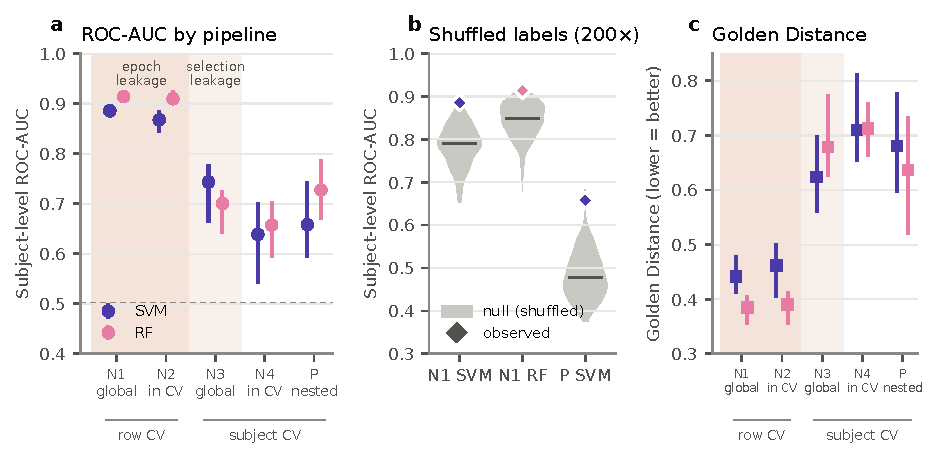
\includegraphics[width=\textwidth]{figures/Fig1_leakage_v2}
  \caption{[CAPTION: Figure 1, leakage.]}
  \label{fig:leakage}
\end{figure}

\begin{figure}
  \centering
  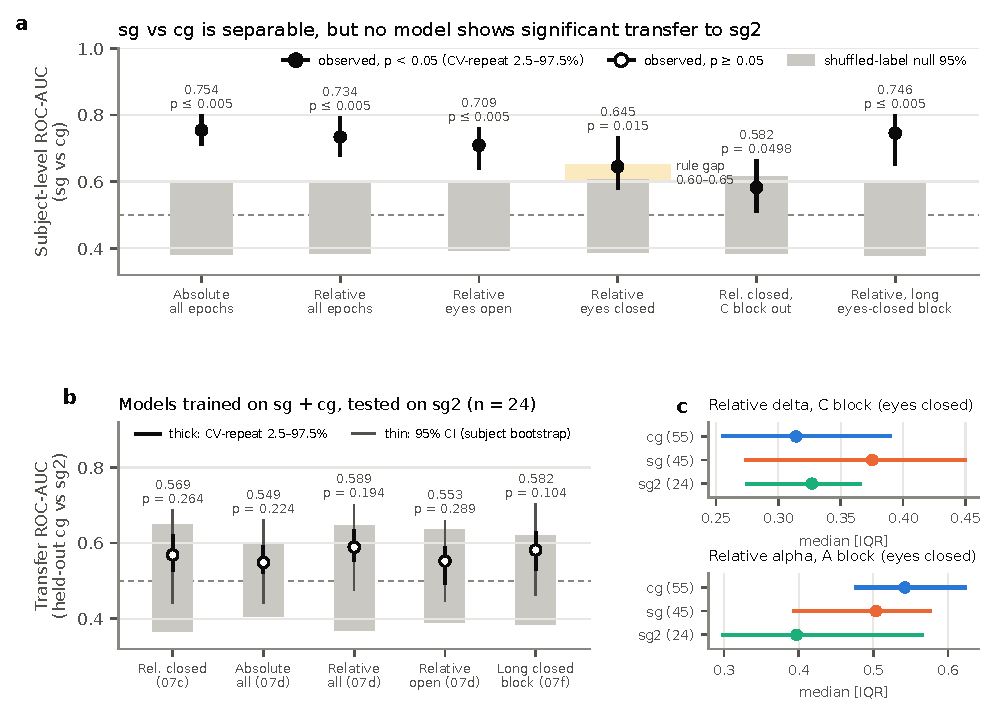
\includegraphics[width=\textwidth]{figures/Fig2_exploratory_cascade_v4}
  \caption{[CAPTION: Figure 2, exploratory cascade and transfer.]}
  \label{fig:cascade}
\end{figure}

\begin{figure}
  \centering
  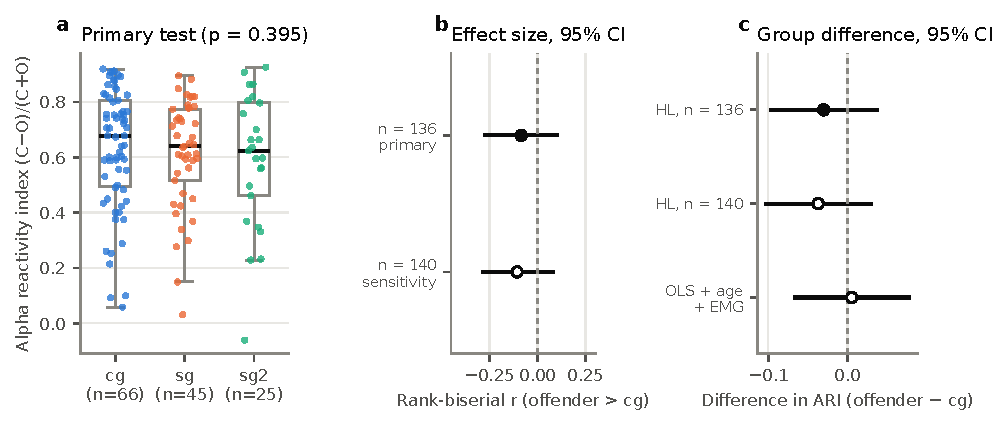
\includegraphics[width=\textwidth]{figures/Fig3_primary_alpha_reactivity_v2}
  \caption{[CAPTION: Figure 3, primary test.]}
  \label{fig:primary}
\end{figure}

\begin{figure}
  \centering
  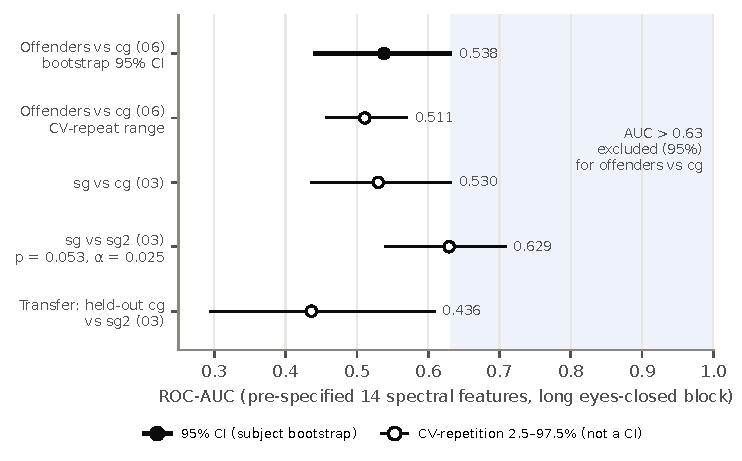
\includegraphics[width=\textwidth]{figures/Fig4_prespecified_null_v2}
  \caption{[CAPTION: Figure 4, ROI-level null.]}
  \label{fig:roi}
\end{figure}

\begin{figure}
  \centering
  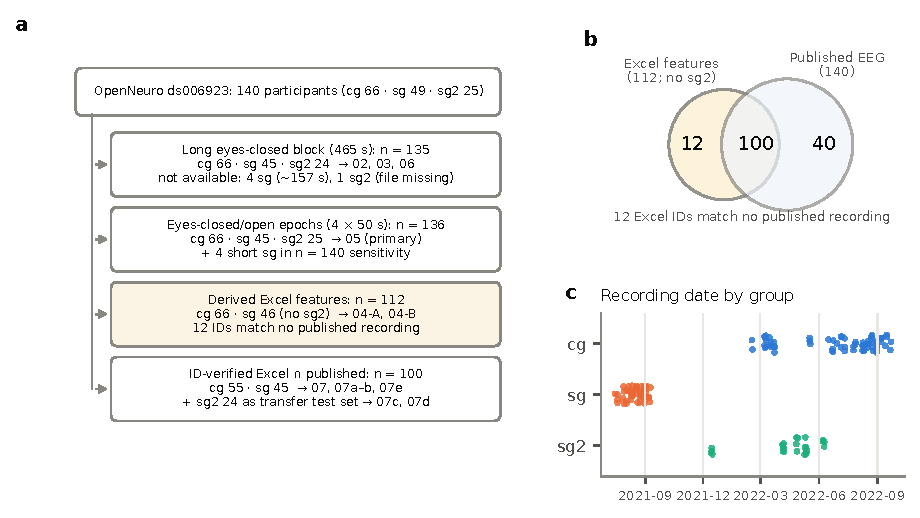
\includegraphics[width=\textwidth]{figures/Fig5_cohort_v2}
  \caption{[CAPTION: Figure 5, cohort and samples.]}
  \label{fig:cohort}
\end{figure}

% ---------------------------------------------------------------- Tables (generated from saved CSV files)
\begin{table}[htbp]
\centering
\caption{[CAPTION]}
\label{tab:Table1}
\footnotesize
\resizebox{\textwidth}{!}{%
\begin{tabular}{p{3.2cm}p{2.6cm}p{2.6cm}p{2.6cm}p{2.6cm}ccl}
\toprule
Variable & sg (n=49) & sg2 (n=25) & offenders (sg + sg2) (n=74) & cg (n=66) & p offenders vs cg & p sg vs sg2 & test \\
\midrule
Age (years) & 17.2 $\pm$ 1.1; 17.0 [17.0--18.0] (n=49) & 16.6 $\pm$ 1.0; 17.0 [16.0--17.0] (n=25) & 17.0 $\pm$ 1.1; 17.0 [16.0--18.0] (n=74) & 16.3 $\pm$ 1.1; 16.0 [16.0--17.0] (n=66) & $<$ 0.001 & 0.031 & Mann--Whitney U \\
Years of education & 8.0 $\pm$ 2.6; 8.0 [6.0--10.0] (n=49) & 7.2 $\pm$ 2.6; 7.0 [6.0--9.0] (n=25) & 7.8 $\pm$ 2.6; 8.0 [6.0--10.0] (n=74) & 10.4 $\pm$ 0.8; 10.0 [10.0--11.0] (n=66) & $<$ 0.001 & 0.272 & Mann--Whitney U \\
Socioeconomic stratum (1--3) & 1.1 $\pm$ 0.3; 1.0 [1.0--1.0] (n=49) & 1.0 $\pm$ 0.0; 1.0 [1.0--1.0] (n=25) & 1.1 $\pm$ 0.3; 1.0 [1.0--1.0] (n=74) & 1.7 $\pm$ 0.5; 2.0 [1.0--2.0] (n=66) & $<$ 0.001 & 0.072 & Mann--Whitney U \\
School dropout & 41/49 (84\%) & 19/25 (76\%) & 60/74 (81\%) & 0/66 (0\%) & $<$ 0.001 & 0.533 & Fisher exact \\
Gang member & 19/49 (39\%) & 4/25 (16\%) & 23/74 (31\%) & 1/66 (2\%) & $<$ 0.001 & 0.063 & Fisher exact \\
Domestic violence & 6/49 (12\%) & 5/25 (20\%) & 11/74 (15\%) & 1/66 (2\%) & 0.005 & 0.492 & Fisher exact \\
Displaced by violence & 5/49 (10\%) & 2/25 (8\%) & 7/74 (9\%) & 3/66 (5\%) & 0.334 & 1.000 & Fisher exact \\
Psychoactive substance use & 36/49 (73\%) & 21/25 (84\%) & 57/74 (77\%) & 12/66 (18\%) & $<$ 0.001 & 0.389 & Fisher exact \\
Alcohol & 25/49 (51\%) & 20/25 (80\%) & 45/74 (61\%) & 12/66 (18\%) & $<$ 0.001 & 0.023 & Fisher exact \\
Marijuana & 34/49 (69\%) & 21/25 (84\%) & 55/74 (74\%) & 0/66 (0\%) & $<$ 0.001 & 0.261 & Fisher exact \\
Cocaine & 29/49 (59\%) & 20/25 (80\%) & 49/74 (66\%) & 0/66 (0\%) & $<$ 0.001 & 0.118 & Fisher exact \\
Age of first use (users) & 13.2 $\pm$ 2.3; 14.0 [13.0--14.0] (n=36) & 13.7 $\pm$ 1.7; 14.0 [13.0--14.0] (n=21) & 13.4 $\pm$ 2.1; 14.0 [13.0--14.0] (n=57) & 14.6 $\pm$ 0.5; 15.0 [14.0--15.0] (n=12) & 0.009 & 0.505 & Mann--Whitney U \\
Violent primary offence (offenders) & 42/49 (86\%) & 6/25 (24\%) & 48/74 (65\%) & -- & -- & $<$ 0.001 & Fisher exact \\
Recidivist (offenders) & 18/49 (37\%) & 6/25 (24\%) & 24/74 (32\%) & -- & -- & 0.306 & Fisher exact \\
Recording clock time (h) & 11.5 $\pm$ 2.3; 10.9 [9.1--14.0] (n=49) & 11.9 $\pm$ 2.2; 11.7 [9.8--14.2] (n=25) & 11.7 $\pm$ 2.2; 10.9 [9.7--14.0] (n=74) & 11.5 $\pm$ 1.7; 10.8 [9.9--13.1] (n=66) & 0.823 & 0.248 & Mann--Whitney U \\
Recording after 14:00 & 14/49 (29\%) & 7/25 (28\%) & 21/74 (28\%) & 6/66 (9\%) & 0.005 & 1.000 & Fisher exact \\
Level of education (coded differently by group; descriptive only) & Basic primary: 13; Basic secondary: 36 & Basic primary: 6; Basic secondary: 19 & Basic primary: 19; Basic secondary: 55 & Basic secondary: 6; High school: 1; Middle school: 57; Technical: 1; University: 1 & -- & -- & none \\
Recording period (first--last month) & 2021-07 -- 2021-09 & 2021-12 -- 2022-06 & 2021-07 -- 2022-06 & 2022-02 -- 2022-09 & -- & -- & none \\
\bottomrule
\end{tabular}
}
\par\smallskip
\begin{minipage}{\textwidth}\raggedright\scriptsize
Notes. Mean $\pm$ SD; median [Q1--Q3] (n with data). p: offenders (sg + sg2) vs cg and sg vs sg2 (test column); $<$ 0.001 shown as such. Source: participants.tsv.
\end{minipage}
\end{table}

\begin{table}[htbp]
\centering
\caption{[CAPTION]}
\label{tab:Table2}
\footnotesize
\resizebox{\textwidth}{!}{%
\begin{tabular}{llllcccccc}
\toprule
Pipeline & CV unit & Feature selection & Row AUC & Subject AUC & Subject balanced accuracy & Subject GD & Shuffled-label null: metric & Null mean [2.5--97.5] & p \\
\midrule
N1 RF & row-wise 10-fold & whole data & 0.87 & 0.91 & 0.80 & 0.38 & row AUC & 0.78 [0.69--0.84] & $\leq$ 0.005 \\
N1 SVM & row-wise 10-fold & whole data & 0.85 & 0.89 & 0.76 & 0.44 & row AUC & 0.73 [0.67--0.80] & $\leq$ 0.005 \\
N2 RF & row-wise 10-fold & within CV & 0.86 & 0.91 & 0.79 & 0.39 & -- & -- & -- \\
N2 SVM & row-wise 10-fold & within CV & 0.83 & 0.87 & 0.74 & 0.46 & -- & -- & -- \\
N3 RF & subject-wise 5-fold & whole data & 0.68 & 0.70 & 0.60 & 0.68 & -- & -- & -- \\
N3 SVM & subject-wise 5-fold & whole data & 0.71 & 0.74 & 0.63 & 0.62 & -- & -- & -- \\
N4 RF & subject-wise 5-fold & within CV & 0.64 & 0.66 & 0.58 & 0.71 & -- & -- & -- \\
N4 SVM & subject-wise 5-fold & within CV & 0.62 & 0.64 & 0.57 & 0.71 & -- & -- & -- \\
P RF & subject-wise 5-fold $\times$ 20, nested & inner loop (k, C) & 0.70 & 0.73 [0.67--0.79] & 0.64 & 0.64 & -- & -- & -- \\
P SVM & subject-wise 5-fold $\times$ 20, nested & inner loop (k, C) & 0.64 & 0.66 [0.59--0.75] & 0.59 & 0.68 & subject AUC & 0.48 [0.40--0.58] & 0.010 \\
\bottomrule
\end{tabular}
}
\par\smallskip
\begin{minipage}{\textwidth}\raggedright\scriptsize
Notes. Published Excel-derived features (CAR\_FREC\_DATS.mat), 112 subjects (cg 66, sg 46); one row per subject $\times$ epoch. N1--N4: 10 CV repeats; P: 20 repeats. Subject AUC/balanced accuracy/GD: row decision values averaged per subject. For P, the bracket gives the 2.5th--97.5th percentile across CV repeats (not a sampling CI). Shuffled-label null: labels permuted at subject level, 200 permutations; smallest attainable p = 1/201 (shown as $\leq$ 0.005). No permutation was run for the remaining cells (--). GD = Golden Distance on [accuracy, sensitivity, specificity, F1], positive class sg; lower is better. The naive pipelines were built in this study to represent a common error; they are not attributed to the data owners.
\end{minipage}
\end{table}

\begin{table}[htbp]
\centering
\caption{[CAPTION]}
\label{tab:Table3}
\footnotesize
\resizebox{\textwidth}{!}{%
\begin{tabular}{lcccccccccc}
\toprule
Analysis & n (offenders / cg) & ARI median, offenders & ARI median [Q1--Q3], cg & U & p & Rank-biserial r [95\% CI] & HL shift [95\% CI] & Adjusted offender coefficient [95\% CI] & p (age) & p (EMG) \\
\midrule
Primary: Mann--Whitney U & 70 / 66 & 0.636 & 0.678 [0.493--0.804] & 2114 & 0.395 & $-$0.08 [$-$0.28, 0.11] & $-$0.03 [$-$0.10, 0.04] & -- & -- & -- \\
Sensitivity: incl. short-recording sg (C1/O1 only) & 74 / 66 & 0.630 & 0.678 [0.493--0.804] & 2182 & 0.279 & $-$0.11 [$-$0.29, 0.09] & $-$0.04 [$-$0.10, 0.03] & -- & -- & -- \\
OLS: ARI $\sim$ offender + age + EMG (HC3) & n = 136 & -- & -- & -- & 0.886 & -- & -- & 0.01 [$-$0.07, 0.08] & 0.032 & 0.050 \\
OLS: rank(ARI) $\sim$ offender + age + EMG (HC3) & n = 136 & -- & -- & -- & 0.988 & -- & -- & $-$0.10 [$-$13.81, 13.60] & 0.033 & 0.169 \\
\bottomrule
\end{tabular}
}
\par\smallskip
\begin{minipage}{\textwidth}\raggedright\scriptsize
Notes. ARI = (C $-$ O)/(C + O), posterior ROI absolute alpha (8--13 Hz) power, eyes closed (C) and open (O) epochs of the first 4 minutes. Two-sided Mann--Whitney U, $\alpha$ = 0.05; rank-biserial r positive when offenders $>$ cg; HL = Hodges--Lehmann shift (offenders $-$ cg, ARI units); CIs bootstrap. OLS rows: HC3 robust SE; the offender coefficient is in ARI units (ARI model) or rank units (rank model); its p is in the p column. The interquartile range of the combined offender group is not recorded in the saved outputs; subgroup descriptives (no test), ARI median [Q1--Q3]: sg (n = 45) 0.640 [0.516--0.774]; sg2 (n = 25) 0.624 [0.461--0.797]; cg (n = 66) 0.678 [0.493--0.804].
\end{minipage}
\end{table}

\begin{table}[htbp]
\centering
\caption{[CAPTION]}
\label{tab:Table4}
\footnotesize
\resizebox{\textwidth}{!}{%
\begin{tabular}{llccccccc}
\toprule
Analysis & Comparison (n) & AUC from mean score [bootstrap 95\% CI] & DeLong 95\% CI & Repeat-mean AUC [2.5--97.5] & Significance threshold (null 97.5th pct.) & p & $\alpha$ & Sensitivity variants, range \\
\midrule
06: offenders vs cg (prespecified null quantification) & offenders (sg + sg2) vs cg (69 / 66) & 0.54 [0.44--0.63] & 0.44--0.64 & 0.51 [0.46--0.57] & -- & -- & -- & -- \\
03(b) reference & sg vs cg (sg 45 / cg 66) & -- & -- & 0.53 [0.43--0.63] & -- & -- & -- & 0.50--0.56 \\
03(a) negative control & sg vs sg2 (sg 45 / sg2 24) & -- & -- & 0.63 [0.54--0.71] & 0.65 & 0.053 & 0.025 & 0.58--0.63 \\
03(b) transfer (within fold) & held-out cg vs sg2 (cg 66 / sg2 24) & -- & -- & 0.44 [0.29--0.61] & 0.65 & 0.771 & 0.025 & 0.42--0.53 \\
\bottomrule
\end{tabular}
}
\par\smallskip
\begin{minipage}{\textwidth}\raggedright\scriptsize
Notes. Features: 14 prespecified ROI-level features from the long eyes-closed block (posterior and global relative band power, aperiodic exponent and offset, IAF). Pipeline: median imputation $\rightarrow$ StandardScaler $\rightarrow$ L2 logistic regression (balanced), outer stratified 5-fold $\times$ 20 repeats, inner 5-fold for C. 06: AUC computed from subject scores averaged over repeats, with class-stratified subject bootstrap and DeLong CIs; repeat-mean AUC with 2.5th--97.5th percentile across repeats (not a sampling CI). 03: 1000 permutations; $\alpha$ = 0.025 per test (prespecified). 03(b) transfer: model trained on sg + cg, AUC of held-out cg vs sg2 within each fold, averaged over 100 folds. Sensitivity range: minimum--maximum over the 7 rows of the 03 sensitivity file (primary and six variants).
\end{minipage}
\end{table}


% ---------------------------------------------------------------- Supplementary material (moves to a separate file at submission)
\clearpage
\section*{Supplementary material (draft placement)}
% Taslak numaralandırma: S1 örneklemler, S2 karar günlüğü (henüz yok), S3 parametreler, S4 keşifsel analizler,
% S5 Excel denetimi, S6 sızıntı duyarlılığı. Son numaralar ilk atıf sırasına göre verilecek.
% sections/supp_note1.tex — Ek not S1 (talimattaki "Kutu 1"), taslak v1 (2026-10-03)
% Kaynak: 04a_excel_audit_v1_2026-10-01_rapor.md §3 ve 04a_excel_audit_v1_2026-10-01_n_points.csv.

\section*{Supplementary note S1. Statistics computed from three values}
\label{sec:suppnote1}

For every band, segment and channel, the spreadsheet files report seven statistics per participant: RMS, standard deviation, minimum, maximum, skewness, kurtosis and power (column names \texttt{RMS}, \texttt{Standarddesv}, \texttt{Minimun}, \texttt{Maximun}, \texttt{Symetry}, \texttt{Kurtosis}, \texttt{Power}). All except power are consistent with having been computed from exactly three values.

\paragraph{Kurtosis.} Let $x_1, x_2, x_3$ be three values that are not all equal, with mean $\bar{x}$ and deviations $d_i = x_i - \bar{x}$, so that $d_1 + d_2 + d_3 = 0$. Let $q = d_1 d_2 + d_1 d_3 + d_2 d_3$. Then
\begin{align*}
\sum_i d_i^2 &= \Big(\sum_i d_i\Big)^2 - 2q = -2q, \\
\sum_{i<j} (d_i d_j)^2 &= q^2 - 2\, d_1 d_2 d_3 \sum_i d_i = q^2, \\
\sum_i d_i^4 &= \Big(\sum_i d_i^2\Big)^2 - 2 \sum_{i<j} (d_i d_j)^2 = 4q^2 - 2q^2 = 2q^2 .
\end{align*}
The population moments are therefore $m_2 = -2q/3$ and $m_4 = 2q^2/3$, and the kurtosis is $m_4/m_2^2 = (2q^2/3)/(4q^2/9) = 3/2$, whatever the three values are. In the spreadsheet files, kurtosis lies between 1.49999 and 1.50001 in every cell.

\paragraph{Skewness.} For $n$ values, the absolute population skewness cannot exceed $(n-2)/\sqrt{n-1}$, which is $1/\sqrt{2} \approx 0.7071$ for $n = 3$. Every absolute skewness in the files is within this bound, and the largest equals it (0.70711).

\paragraph{Reconstruction.} If the standard deviation $s$ is the sample standard deviation (denominator $n-1$), the mean of three values follows from the RMS as $\bar{x} = \sqrt{\mathrm{RMS}^2 - 2s^2/3}$ (all values are positive; the smallest is 0.109), and the middle value is $3\bar{x} - \min - \max$. The three values reconstructed in this way reproduce the reported skewness (median absolute error $2 \times 10^{-7}$; 99th percentile $1 \times 10^{-6}$) and standard deviation (median relative error $3 \times 10^{-8}$), and the middle value lies between the minimum and the maximum in every cell. If the population standard deviation is assumed instead, the middle value falls outside this range in 52\% of cells.

\paragraph{Power.} Power is not a function of the same three values: the ratio of power to RMS$^2$ varies across cells (median 0.58, interquartile range 1.0), and the correlation between log power and log RMS is 0.61.

Whether the three values are frequency points or time windows cannot be determined, because the code that produced the files is not part of the dataset. Kurtosis carries no information, and the other five statistics are different summaries of the same three values.


\renewcommand{\thetable}{S\arabic{table}}
\renewcommand{\thefigure}{S\arabic{figure}}
\setcounter{table}{0}
\begin{table}[htbp]
\centering
\caption{[CAPTION]}
\label{tab:TableSn}
\footnotesize
\resizebox{\textwidth}{!}{%
\begin{tabular}{p{3.5cm}p{3.8cm}ccccp{5cm}}
\toprule
Analysis & Data segment & cg & sg & sg2 & Total & Exclusions / notes \\
\midrule
01 Data audit & all files & 66 & 49 & 25 & 140 & -- \\
02 Features / 03 / 06 & long eyes-closed block, 465 s & 66 & 45 & 24 & 135 & 4 sg ($\sim$157 s, no long block), sub-1084sg2 (data file missing) \\
03 (a) sg vs sg2 & long block & 0 & 45 & 24 & 69 & as 02 \\
03 (b) sg+cg $\rightarrow$ sg2 transfer & long block & 66 & 45 & 24 & 135 & as 02 \\
04-A / 04-B Excel features & Excel C\_1, O\_1, C\_2, O\_2 (derived) & 66 & 46 & 0 & 112 & Excel cohort: 12 IDs not in published data; sg2 absent \\
04-B sensitivity (ID-verified) & Excel & 55 & 45 & 0 & 100 & 12 unverified Excel IDs \\
05 Alpha reactivity (primary) & 4 $\times$ 50 s eyes-closed/open epochs & 66 & 45 & 25 & 136 & 4 sg with 2 epochs (included only in n = 140 sensitivity) \\
06 Offenders vs cg & long block & 66 & 45 & 24 & 135 & as 02 \\
07 / 07a / 07b / 07e & epochs (07--07b) or long block (07e) & 55 & 45 & 0 & 100 & restricted to Excel $\cap$ published, ID-verified \\
07c / 07d transfer test set & same epochs as training (07c: eyes closed; 07d: all / eyes open) & 0 & 0 & 24 & 24 & sub-1084sg2 excluded (25 in extra row) \\
07f transfer test set & long eyes-closed block, 465 s (4 $\times$ 116.25 s), as 07e & 0 & 0 & 24 & 24 & sub-1084sg2 has no long block (data file missing); training set as 07e (cg 55, sg 45) \\
07g 95\% CIs (no new model) & as 07--07f & 55 & 45 & 24 & 124 & source models: cg 55 + sg 45; transfer: held-out cg (55) vs sg2 24; descriptive sensitivity without sub-1105sg2 and sub-1114sg2 (sg2 22) \\
\bottomrule
\end{tabular}
}
\end{table}

\setcounter{table}{2}
\begin{table}[htbp]
\centering
\caption{[CAPTION]}
\label{tab:TableS3}
\footnotesize
\resizebox{\textwidth}{!}{%
\begin{tabular}{p{3.2cm}p{6.5cm}cccl}
\toprule
Item & Setting & sg & sg2 & cg & Source \\
\midrule
\multicolumn{6}{l}{\textit{A. Parameters (prespecified)}} \\
Segment & Fixed 465 s from the 3rd eyes-closed marker + 5 s; two halves H1, H2 (232.5 s each) &  &  &  & CLAUDE.md, line 46 \\
PSD & Welch, 4 s Hann window, 50\% overlap (0.25 Hz resolution) &  &  &  & CLAUDE.md, line 47 \\
Bands (relative power) & delta 1--4, theta 4--8, alpha 8--13, beta 13--30 Hz; denominator = 1--30 Hz total; gamma not a feature (EMG control only) &  &  &  & CLAUDE.md, line 48 \\
Aperiodic fit (FOOOF) & fooof 1.1; primary: aperiodic mode 'fixed', 3--30 Hz &  &  &  & CLAUDE.md, line 49 \\
Aperiodic fit, sensitivity & 'knee' mode, 2--30 Hz; sensitivity analysis only, no post hoc choice &  &  &  & CLAUDE.md, line 50 \\
IAF & Primary: strongest FOOOF peak in 7--13 Hz; secondary: centre of gravity in 7--13 Hz of the aperiodic-removed spectrum; no PSD argmax &  &  &  & CLAUDE.md, line 51 \\
EMG index & Slope of log10 PSD vs log10 f, 30--40 Hz (flatter/positive = more muscle); covariate in group analyses &  &  &  & CLAUDE.md, line 53 \\
Channel exclusion & Primary FOOOF R$^{2}$ $<$ 0.9 OR EMG index robust z $>$ 3 (median + 3$\cdot$1.4826$\cdot$MAD, one-sided); determined on the full segment, same set for halves &  &  &  & CLAUDE.md, line 54 \\
ROI features & Computed from the mean spectrum of the retained channels &  &  &  & CLAUDE.md, line 55 \\
Atypical-spectrum rule & $>$ 25\% of channels ($>$ 32/128) excluded $\rightarrow$ subject flagged; only the EMG rule applied, ROI from all remaining channels; included in primary, excluded in sensitivity analyses &  &  &  & CLAUDE.md, line 59 \\
Vigilance & Theta/alpha ratio in 30 s windows; slope (log10 ratio per min) as vigilance index; features also for H1 and H2 &  &  &  & CLAUDE.md, line 56 \\
EMG index caveat & Includes the roll-off of the preprocessing low-pass FIR filter; valid as a relative index only &  &  &  & 02\_features\_v2\_rapor\_2026-10-01.md, line 51 \\
\midrule
\multicolumn{6}{l}{\textit{B. QC summary, median [Q1--Q3]}} \\
Subjects processed (n) &  & 45 & 24 & 66 & 02\_features\_v2\_2026-10-01\_subject\_qc.csv \\
EMG index (channel median, all channels) &  & $-$1.88 [$-$2.37, $-$1.38] & $-$2.56 [$-$3.04, $-$1.71] & $-$2.04 [$-$2.52, $-$1.41] & 02\_descriptive\_by\_group\_v2\_2026-10-01.csv \\
Excluded channels, total &  & 3 [1--7] & 3.5 [1--8] & 3 [1--6] & 02\_descriptive\_by\_group\_v2\_2026-10-01.csv \\
\ldots{} due to R$^{2}$ $<$ 0.9 &  & 0 [0--3] & 0 [0--4.25] & 0 [0--1] & 02\_descriptive\_by\_group\_v2\_2026-10-01.csv \\
\ldots{} due to EMG z $>$ 3 &  & 2 [0--3] & 1 [0--4] & 1 [0--4] & 02\_descriptive\_by\_group\_v2\_2026-10-01.csv \\
FOOOF R$^{2}$, channel median &  & 0.989 [0.987--0.990] & 0.985 [0.983--0.990] & 0.990 [0.986--0.992] & 02\_descriptive\_by\_group\_v2\_2026-10-01.csv \\
FOOOF R$^{2}$, posterior ROI &  & 0.991 [0.988--0.994] & 0.983 [0.976--0.992] & 0.990 [0.984--0.994] & 02\_descriptive\_by\_group\_v2\_2026-10-01.csv \\
Theta/alpha slope, global (log10 ratio/min) &  & 0.014 [$-$0.006, 0.037] & 0.020 [0.008--0.029] & 0.026 [0.005--0.059] & 02\_descriptive\_by\_group\_v2\_2026-10-01.csv \\
Theta/alpha slope, posterior &  & 0.009 [$-$0.007, 0.024] & 0.017 [0.010--0.032] & 0.029 [0.007--0.070] & 02\_descriptive\_by\_group\_v2\_2026-10-01.csv \\
Atypical-spectrum subjects ($>$ 32 channels excluded) &  & 0 & 2 & 0 & 02\_features\_v2\_2026-10-01\_subject\_qc.csv \\
\bottomrule
\end{tabular}
}
\par\smallskip
\begin{minipage}{\textwidth}\raggedright\scriptsize
Notes. Panel A: parameters fixed before any group comparison (CLAUDE.md, 'prespecified primary analysis'); line numbers refer to the files at commit time. Panel B: full 465 s segment, primary FOOOF fit; descriptive only, no group test. Subjects without a long eyes-closed block or with a missing data file are not included (Table S-n).
\end{minipage}
\end{table}

\begin{table}[htbp]
\centering
\caption{[CAPTION]}
\label{tab:TableS4}
\footnotesize
\resizebox{\textwidth}{!}{%
\begin{tabular}{lp{2.6cm}p{2.6cm}cccccccccccc}
\toprule
Analysis & Data & Comparison & AUC [repeat range] & AUC (mean score) & 95\% CI & Null mean & p & BA & GD & Sen & Spe & F1 & sg2 classified offender & AUC excl. atypical sg2 \\
\midrule
07 A & log10 absolute band power, all epochs & sg vs cg (n = 45 / 55) & 0.75 [0.71--0.80] & 0.77 & 0.67--0.86 & 0.48 & $\leq$ 0.005 & 0.67 & 0.57 & 0.57 & 0.76 & 0.61 & -- & -- \\
07 B & relative band power, all epochs & sg vs cg (n = 45 / 55) & 0.73 [0.67--0.79] & 0.80 & 0.71--0.89 & 0.48 & $\leq$ 0.005 & 0.65 & 0.61 & 0.49 & 0.81 & 0.57 & -- & -- \\
07a closed & B, eyes-closed epochs (2 $\times$ 50 s) & sg vs cg (n = 45 / 55) & 0.64 [0.58--0.73] & 0.71 & 0.60--0.81 & 0.48 & 0.015 & 0.60 & 0.66 & 0.47 & 0.73 & 0.52 & -- & -- \\
07a open & B, eyes-open epochs (2 $\times$ 50 s) & sg vs cg (n = 45 / 55) & 0.71 [0.64--0.76] & 0.77 & 0.67--0.86 & 0.49 & $\leq$ 0.005 & 0.65 & 0.59 & 0.58 & 0.72 & 0.60 & -- & -- \\
07b & B, eyes closed, C block removed & sg vs cg (n = 45 / 55) & 0.58 [0.51--0.67] & 0.61 & 0.49--0.72 & 0.48 & 0.050 & 0.56 & 0.72 & 0.41 & 0.71 & 0.46 & -- & -- \\
07e & B, long eyes-closed block (4 $\times$ 116.25 s) & sg vs cg (n = 45 / 55) & 0.75 [0.65--0.80] & 0.78 & 0.69--0.87 & 0.48 & $\leq$ 0.005 & 0.66 & 0.60 & 0.51 & 0.81 & 0.58 & -- & -- \\
07c & B, eyes-closed epochs & held-out cg vs sg2 (n = 55 / 24), within fold & 0.57 [0.53--0.62] & -- & 0.44--0.69 & 0.51 & 0.264 & -- & -- & -- & -- & -- & 0.44 & 0.54 \\
07d A all & A, all epochs & held-out cg vs sg2 (n = 55 / 24), within fold & 0.55 [0.52--0.59] & -- & 0.44--0.66 & 0.50 & 0.224 & -- & -- & -- & -- & -- & 0.19 & 0.57 \\
07d B all & B, all epochs & held-out cg vs sg2 (n = 55 / 24), within fold & 0.59 [0.55--0.64] & -- & 0.48--0.70 & 0.51 & 0.194 & -- & -- & -- & -- & -- & 0.33 & 0.56 \\
07d B open & B, eyes-open epochs & held-out cg vs sg2 (n = 55 / 24), within fold & 0.55 [0.49--0.59] & -- & 0.45--0.66 & 0.51 & 0.289 & -- & -- & -- & -- & -- & 0.35 & 0.53 \\
07f & B, long eyes-closed block & held-out cg vs sg2 (n = 55 / 24), within fold & 0.58 [0.53--0.63] & -- & 0.46--0.70 & 0.50 & 0.104 & -- & -- & -- & -- & -- & 0.30 & 0.56 \\
\bottomrule
\end{tabular}
}
\par\smallskip
\begin{minipage}{\textwidth}\raggedright\scriptsize
Notes. All exploratory; p values unadjusted; 200 permutations (smallest attainable p = 1/201, shown as $\leq$ 0.005). Source models (sg vs cg): AUC = mean over 20 repeats, bracket = 2.5th--97.5th percentile across repeats; 95\% CI = class-stratified subject bootstrap of the AUC from repeat-averaged subject scores (AUC mean score). Transfer models (held-out cg vs sg2, within fold): AUC = mean of 100 fold AUCs; 95\% CI = weighted subject bootstrap. 'AUC excl. atypical sg2': descriptive, without the two atypical-spectrum sg2 subjects. BA, GD, Sen, Spe, F1 at subject level, positive class sg. Smaller GD is better.
\end{minipage}
\end{table}

\begin{table}[htbp]
\centering
\caption{[CAPTION]}
\label{tab:TableS5}
\footnotesize
\begin{tabular}{p{3.5cm}p{9cm}p{3.5cm}}
\toprule
Item & Finding & Source \\
\midrule
File structure & 2048 files = 4 bands (ALFA, BETA, DELTA, THETA) $\times$ 4 condition-epochs (C\_1, C\_2, O\_1, O\_2) $\times$ 128 channels; 7 statistics per file & 04a\_excel\_audit\_v1\_2026-10-01\_structure.csv \\
Empty (0-byte) files & 1: FR\_Dats\_band\_THETA\_EP\_C\_2\_can\_B12.xlsx (values available in CAR\_FREC\_DATS.mat) & 04a\_excel\_audit\_v1\_2026-10-01\_structure.csv \\
Subjects in the Excel files & 112 (cg 66, Label = 0; sg 46, Label = 1); no sg2 & 04a\_excel\_audit\_v1\_2026-10-01\_ids.csv \\
Excel IDs absent from the published dataset & 12: cg\_rs\_2013, cg\_rs\_2024, cg\_rs\_2025, cg\_rs\_2027, cg\_rs\_2035, cg\_rs\_2039, cg\_rs\_2041, cg\_rs\_2058, cg\_rs\_2069, cg\_rs\_2073, cg\_rs\_2076, sg\_rs\_1011 & 04a\_excel\_audit\_v1\_2026-10-01\_ids.csv \\
Published subjects absent from the Excel files & 40 (sg2 25, sg 4, cg 11) & 01\_data\_audit\_v2\_2026-10-01.csv; 04a\_excel\_audit\_v1\_2026-10-01\_ids.csv \\
Statistics computed from 3 values & Kurtosis 1.49999--1.50001 in every cell (population kurtosis of any 3 unequal values = 1.5); max absolute skewness = 0.707107 (bound for 3 values: 1/$\surd$2) & 04a\_excel\_audit\_v1\_2026-10-01\_n\_points.csv \\
SD convention & Sample SD (n $-$ 1): reconstructed middle value within [Min, Max] in 100.0\% of cells vs 47.7\% with population SD & 04a\_excel\_audit\_v1\_2026-10-01\_n\_points.csv \\
ID verification (log-power profile correlation) & Best match = own ID in 100/100; r with own ID median 0.915 (range 0.723--0.984); smallest margin over the second-best match 0.151 & 04a\_excel\_audit\_v1\_2026-10-01\_id\_match.csv \\
Unknown Excel IDs & None of the 12 matched a published recording: best r 0.25--0.66 & 04a\_excel\_audit\_v1\_2026-10-01\_id\_match.csv \\
\bottomrule
\end{tabular}
\par\smallskip
\begin{minipage}{\textwidth}\raggedright\scriptsize
Notes. Excel feature files are part of the published dataset (code/ folder); no Excel result can be reproduced from the published EEG because the cohorts differ. ID verification: z-scored log-power profiles (4 bands $\times$ 4 epochs $\times$ 128 channels) from the Excel files vs. the same profile recomputed from the published acq-epochs files; Pearson correlation.
\end{minipage}
\end{table}

\begin{table}[htbp]
\centering
\caption{[CAPTION]}
\label{tab:TableS_leak}
\footnotesize
\begin{tabular}{lcccc}
\toprule
Variant & N1 RF & N1 SVM & P RF & P SVM \\
\midrule
Primary (reference) & 0.91 & 0.89 & 0.73 & 0.66 \\
ID-verified subjects only & 0.92 & 0.84 & 0.69 & 0.62 \\
Kurtosis features removed & 0.91 & 0.89 & 0.73 & 0.68 \\
Eyes-closed epochs only & 0.86 & 0.78 & 0.65 & 0.60 \\
\bottomrule
\end{tabular}
\par\smallskip
\begin{minipage}{\textwidth}\raggedright\scriptsize
Notes. ID-verified: the 100 Excel subjects whose published EEG matched their own ID (Table S5). Pipelines as in Table 2; N1 = naive (row-wise CV, selection on whole data), P = correct nested subject-wise CV.
\end{minipage}
\end{table}

\setcounter{figure}{0}

\begin{figure}
  \centering
  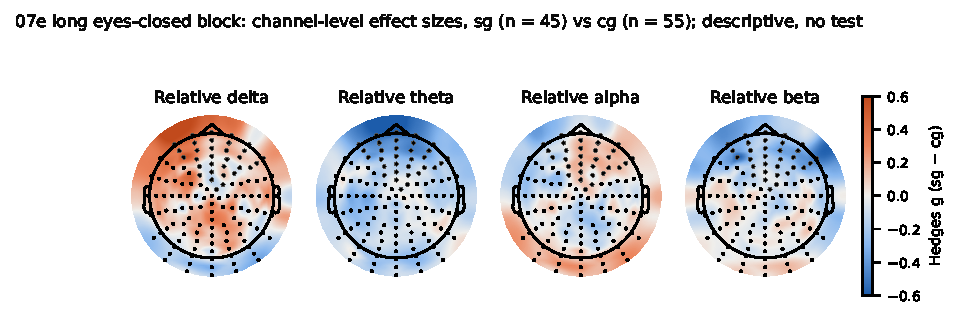
\includegraphics[width=\textwidth]{figures/FigS_07e_feature_map_v1}
  \caption{[CAPTION: Figure S1, 07e feature map.]}
  \label{fig:S07e}
\end{figure}

% ---------------------------------------------------------------- Back matter
\ack{We thank the creators of the dataset for making their recordings openly available. During the preparation of this manuscript, the authors used Claude Code (Anthropic; model Claude Opus 5.5) to write and run the analysis code, and Claude Opus 5.5 (Anthropic) to audit the analyses and to support the writing. The authors reviewed, validated and critically assessed all AI-assisted outputs and take full responsibility for the content of the manuscript.}

\funding{This research received no specific grant from any funding agency in the public, commercial or not-for-profit sectors.}

\roles{Mesut Melek: conceptualization, methodology, software, formal analysis, writing -- review \& editing. Negin Melek: methodology, software, formal analysis, writing -- original draft.}

\data{The EEG data are openly available on OpenNeuro (ds006923, version 1.0.0) \cite{Polo2025ds006923}. The analysis code, analysis log and result files are available at [REPOSITORY / ZENODO DOI].}

\suppdata{[SUPPLEMENTARY FILES: tables S1--S5, figure S1, analysis log (table S2), commit records.]}

\bibliographystyle{unsrt}
\bibliography{refs}

\end{document}
